% Anonymous submission (English version) for ASCAT 2027 -- Indian Summer School on Cellular Automata 2026
% Springer LNCS format (llncs.cls). Max 12 pages. Deadline: 2026/10/09.
%
\documentclass[runningheads,a4paper]{llncs}
%
\usepackage[T1]{fontenc}
\usepackage{newtxtext}
\usepackage[varvw]{newtxmath}
\usepackage{graphicx}
\usepackage{subcaption}
\graphicspath{{figures/}}
\usepackage{algorithm}
\usepackage{algpseudocode}
\usepackage{comment}
% Sorts and compresses the numbers inside each citation, e.g. [1--3].
\usepackage{cite}
% Allows extra stretch for paragraphs that would otherwise be overfull.
\setlength{\emergencystretch}{1em}

%
% To display URLs in blue roman font according to Springer's eBook style:
\usepackage{hyperref}
\usepackage{color}
\renewcommand\UrlFont{\color{blue}\rmfamily}
\urlstyle{rm}
%
\begin{document}
%
\title{Spectral Moments with Attractor Mass: A Similarity Index for One-Dimensional Cellular Automata}
\titlerunning{Spectral Moments with Attractor Mass}
%
% Anonymous version for the double-blind review of ASCAT 2027.
% Author names, ORCID, affiliations, e-mail and acknowledgments are removed.
\author{Anonymous Author(s)}
%
\authorrunning{Anonymous}
%
\institute{Anonymous Institution}
%
\maketitle
%
% Required first-page footer (unnumbered footnote).
{\renewcommand\thefootnote{}\footnotetext{This work is done as a project in
the Indian Summer School on Cellular Automata 2026.}\addtocounter{footnote}{-1}}
%
\begin{abstract}
% Abstract text (150--250 words). Keywords are set in main.tex.
Classifications of cellular automata group rules by their behavior, but they do not measure how similar the rules are. We look for a similarity index based on the evolution that allows rules to be compared, even when they have different numbers of states or neighbors. First, we define four exact relations (state permutation, mirror, state reduction and neighborhood reduction), which reduce the 256 rules of the elementary cellular automata (ECA) to 81 classes. Then we compare the transition graph on a ring of $n$ cells: its canonical form, together with the quotient by translations, distinguishes the 88 classes under permutation and mirror with only 6 cells, but the comparison is binary. As a gradual measure, we propose spectral moments with attractor mass, a fixed-length vector that, unlike the eigenvalues and the spectral moments, counts how many configurations reach each attractor and in how many steps. With the cosine distance, this vector distinguishes 86 of the 88 classes (87 together with the quotient), including rules 0 and 8, and gives zero distance to the relations that preserve the graph and, in the quotient, to those that differ by a translation, but it does not identify state reduction. Moreover, it depends on the size of the space, and it groups the ECA into four families according to the dominant period of their attractors.


\keywords{Cellular automata \and Elementary cellular automata
\and Similarity index \and Transition graph \and Spectral moments
\and Basins of attraction.}
\end{abstract}
%
% ---- Body: one file per section in sections/ ----
\section{Introduction}

Cellular automata are discrete dynamical systems that have been used to model complex systems~\cite{Torres2025_complejo,sole1996_cs_caos,Hoekstra2010_cs_ca}: from very simple local rules they produce behaviors that range from convergence to a homogeneous, easily predictable state to chaotic dynamics~\cite{wolfram1982_ca,Wolfram2002_nks}. To distinguish these behaviors, several classifications have been proposed, such as Wolfram's four classes~\cite{Wolfram2002_nks}, the classification of Li and Packard~\cite{li1990_structure} and others reviewed by Martínez~\cite{genaro2013_class}, or the set of \emph{life-like} rules~\cite{lifewiki_life}. But how similar are the rules within the same class? And how different are they from the rules of another class?

Apart from directly comparing their exact behavior, classifications are the only measure to decide whether two rules are alike, and both give a binary answer. The purpose of this research is to define a method to compare the behavior of any two rules, even if they have different numbers of states or neighbors, and to measure their degree of similarity.

We first identify the exact relations that exist between rules of different domains (Section~\ref{sec:inheritance}) and use them as a reference to validate the proposed methods. We then compare the transition graph through its canonical form (Section~\ref{sec:structural}) and propose spectral methods that represent each rule by a vector (Section~\ref{sec:spectral}): the eigenvalues, the spectral moments and the spectral moments with attractor mass. Finally, we evaluate this last method on rules from different domains, on spaces of different sizes, and by clustering the elementary rules (Section~\ref{sec:experiments}).

\section{Preliminaries}

A cellular automaton is a collection of cells arranged in a lattice, where each cell takes a state from a finite set. The system evolves in discrete time steps and, at each step, all cells update their state synchronously as a function of the states of their neighbors~\cite{weisstein2002_ca,wolfram1982_ca,fsancho2016_ca}.

\begin{definition}
\label{def:ca}
A cellular automaton is a 4-tuple $(\mathcal{L}, \mathcal{S}, \mathcal{N}, \mathcal{R})$ where:
\begin{itemize}
    \item $\mathcal{L} \subseteq \mathbb{Z}^D$ is the $D$-dimensional cellular space; each cell is identified by its position $\vec{i} \in \mathcal{L}$.

    \item $\mathcal{S} = \{0, 1, \dots, q-1\}$ is the finite set of $q$ states. The state of cell $\vec{i}$ at time $t$ is denoted by $\sigma_{\vec{i}}(t) \in \mathcal{S}$.

    \item $\mathcal{N} = (\vec{v}_1, \dots, \vec{v}_m)$ is the ordered tuple of the $m$ displacement vectors that define the neighborhood: the neighbors of $\vec{i}$ are the cells $\vec{i} + \vec{v}_j$, with $j = 1, \dots, m$.

    \item $\mathcal{R} : \mathcal{S}^m \to \mathcal{S}$ is the local rule, which assigns the new state of a cell from the states of its $m$ neighbors:
    \[
    \sigma_{\vec{i}}(t + 1) = \mathcal{R}\left( \sigma_{\vec{i} + \vec{v}_1}(t), \dots, \sigma_{\vec{i} + \vec{v}_m}(t) \right).
    \]
\end{itemize}
\end{definition}

The order of the tuple $\mathcal{N}$ matters: it determines the numbering of the rules and allows us to define relations such as mirror rules (Section~\ref{subsection:rules_same_domain}).

\subsection{Space, neighborhoods and rules}

In practice, the cellular space is restricted by open boundaries, which assign a fixed state to the missing neighbors, or periodic ones, which take them from the opposite boundary~\cite{bhattacharjee2019_ca,ponce2015_ca}. Throughout this work we always use periodic boundaries: in one dimension, the space is a ring of $n$ cells, $\mathcal{L} = \mathbb{Z}_n$, and with radius $r$ the neighborhood contains the $m = 2r + 1$ cells at distance at most $r$, including the cell itself.

The elementary cellular automaton (ECA) has $q = 2$, radius $r = 1$ ($m = 3$) and rule $\mathcal{R} : \{0,1\}^3 \to \{0,1\}$. There are $q^{m} = 2^3 = 8$ possible neighborhood patterns and each one is assigned a new state, so the total number of rules is $q^{q^{m}} = 2^8 = 256$. Each rule is identified by a decimal number obtained by reading, as a binary number, the states assigned to the patterns $111, 110, \dots, 000$~\cite{Wolfram2002_nks}. In general, we denote by $r_{q,m}$ the rule number $r$ with $q$ states and $m$ neighbors, numbered in the same way in base $q$; thus, the ECA are the rules $r_{2,3}$. When $m$ is even the neighborhood cannot be symmetric: with $m = 2$ we use the cells $(i-1, i)$, which is the \textit{Mathematica} convention for radius $r = 1/2$.

\subsection{Global function and transition graph}

Let $\mathcal{C} = \mathcal{S}^{\mathcal{L}}$ be the set of configurations, with $N = |\mathcal{C}| = q^{|\mathcal{L}|}$. The global function $F : \mathcal{C} \to \mathcal{C}$ applies the local rule to all cells synchronously. The transition graph $G_F = (\mathcal{C}, E)$ has one node per configuration and a directed edge $\sigma \to F(\sigma)$. Since $F$ is a function, every node has out-degree 1 (a functional graph). Each connected component contains exactly one cycle, the attractor, with transient trees hanging from it; together they form its basin of attraction. For each $x \in \mathcal{C}$ we define its period $p(x)$ as the length of the cycle it reaches, and its height $h(x)$ as the minimum number of steps needed to reach it ($h(x) = 0$ if $x$ is periodic). Configurations without a predecessor are known as Garden of Eden configurations.

\subsection{Quotient by translations}
\label{subsec:quotient}

Let $T$ be the translation by one position in $\mathcal{L}$ (a rotation of the ring $\mathbb{Z}_n$). With periodic boundaries, $F \circ T = T \circ F$, so two configurations that differ by a translation have equivalent trajectories. This allows us to build the quotient graph, whose nodes are the classes of configurations under translation and whose edges are $[x] \to [F(x)]$. All configurations in the same class have the same height, and the number of nodes drops to approximately $N/|\mathcal{L}|$. In the quotient graph each class counts as a single node, so the proportions computed on it are normalized by the number of classes.

\section{Exact relations: Inheritance properties}
\label{sec:inheritance}

This method arises as an extension of the well-known equivalence criteria: state permutation and mirror rules. We suggest that there are additional relations between rules of different spaces. For example, rule 0 always has the same behavior regardless of the number of states, the size of the neighborhood or the dimension. This raises the following question: what are the similarity criteria between rules of different spaces?

To this end, we call the domain of a rule the 3-tuple of dimension, states and neighborhood on which it is defined. Two rules belong to the same domain if they share all three elements.

\subsection{Rules in the same domain}
\label{subsection:rules_same_domain}

To compare the behavior of rules in the same domain we can apply state permutation and mirror rules, which in ECA reduce the 256 rules to 88 classes \cite{genaro2013_class}.

Let $\mathcal{A}_1$ and $\mathcal{A}_2$ be two cellular automata with the same domain, and let $(x_1, \dots, x_m) \in \mathcal{S}^m$ be the state of the neighborhood. We say that $\mathcal{A}_1$ and $\mathcal{A}_2$ are equivalent if one of the following conditions holds:

\begin{itemize}
    \item \textbf{State permutation}: there is a bijection of states $\pi : \mathcal{S} \to \mathcal{S}$ such that
    \[
    \mathcal{R}_2(x_1, \dots, x_m) = \pi\left( \mathcal{R}_1\left( \pi^{-1}(x_1), \dots, \pi^{-1}(x_m) \right) \right), \quad \forall (x_1, \dots, x_m) \in \mathcal{S}^m.
    \]
    That is, if we relabel all the states, the structure remains the same. For $\mathcal{S} = \{0, 1\}$, the only non-trivial one is $\pi(x) = 1 - x$, which simply swaps the two states.

    \item \textbf{Mirror rules}: let $M : \mathcal{S}^m \to \mathcal{S}^m$ be the reflection of the neighborhood,
    $M(x_1, \dots, x_m) = (x_m, \dots, x_1)$. We say that $\mathcal{A}_2$ is the mirror rule of $\mathcal{A}_1$ if
    \[
    \mathcal{R}_2(x_1, \dots, x_m) = \mathcal{R}_1\left( M(x_1, \dots, x_m) \right).
    \]
    That is, if we reflect the initial configuration, evolve it with $\mathcal{A}_1$ and reflect the result, we obtain exactly the evolution of $\mathcal{A}_2$.
\end{itemize}

\subsection{State reduction}

Let $\mathcal{A}$ be a rule. State reduction is possible when there are two states $a \neq b \in \mathcal{S}$ that satisfy the following conditions:
\begin{enumerate}

    \item State $a$ is never produced by the rule: $\mathcal{R}(x_1, \dots, x_m) \neq a, \; \forall (x_1, \dots, x_m) \in \mathcal{S}^m$.
    \item State $a$ behaves like $b$ in every position of the neighborhood: $\mathcal{R}(x_1, \dots,a, \dots, x_m) = \mathcal{R}(x_1, \dots,b,\dots, x_m)$.
\end{enumerate}
Then the reduced automaton is $\mathcal{A}' = (\mathcal{L}, \mathcal{S}', \mathcal{N}, \mathcal{R}')$ with $\mathcal{S}' = \mathcal{S} \setminus \{a\}$.

The justification is as follows: since state $a$ is never produced, it can only appear in the initial condition, and since its transitions coincide with those of $b$, both have the same behavior for every configuration $\sigma$. Therefore, from the first step on, the evolution of $\mathcal{A}$ is exactly that of $\mathcal{A}'$.

\subsection{Neighborhood reduction}

Neighborhood reduction is possible when the state of a neighbor does not affect the transition, that is, there is an index $j$ such that
\[
\mathcal{R}(x_1, \dots, x_j, \dots, x_m) = \mathcal{R}(x_1, \dots, x_j', \dots, x_m), \quad \forall (x_1, \dots, x_m) \in \mathcal{S}^m, \; \forall x_j' \in \mathcal{S}.
\]
Then the reduced automaton is $\mathcal{A}' = (\mathcal{L}, \mathcal{S}, \mathcal{N}', \mathcal{R}')$ with $\mathcal{N}' = \mathcal{N} \setminus \{\vec{v}_j\}$.

If the removed neighbor is not at one of the ends, the neighborhood is adjusted so that it is contiguous with $m - 1$ cells. For the purposes of this research, this equivalence is applied to any neighbor, under the hypothesis that changing the position of the neighbors only transforms the space of the evolution and not the behavior. With this relation, ECA drops to 81 classes, a range we consider acceptable.

\subsection{Equivalence classes}

With these four relations (state permutation, mirror, state reduction and neighborhood reduction) it is possible to relate rules from different domains. Applying them iteratively builds a relation graph whose connected components are the equivalence classes. Although this classification is still binary (two rules either are or are not equivalent), it serves as a reference to validate the following methods: if two rules are equivalent, their similarity index should be one.

\section{Structural comparison of transition graphs}
\label{sec:structural}

The relations obtained in Section~\ref{sec:inheritance} depend only on the rule vector. As an alternative, we propose to compare the global dynamics: we define a finite periodic space of $n$ cells, which contains $N = |\mathcal{S}|^n$ configurations. By evolving each of them, we obtain the transition graph $G_F$ of the rule.

As a parallel method, all the translations of a configuration (Section~\ref{subsec:quotient}) are considered a single node, which yields a quotient graph with approximately $|\mathcal{S}|^n / n$ nodes.

We then say that two rules have the same behavior if their transition graphs have the same topology, that is, if they are isomorphic.

\subsection{Isomorphism and canonical form}

The isomorphism comparison identifies exactly the rules related by state permutation and mirror rules, which confirms that the transition graph captures the similarity between rules.

This process is computationally expensive. As an alternative, we use the canonical form of the transition graph: a topological encoding of a graph that does not depend on the node labels, so that two graphs are isomorphic if and only if their canonical forms are equal. The canonical form is built with Algorithm~\ref{alg:canonnical_form}.

\begin{algorithm}
\caption{Canonical form of a transition diagram}
\begin{algorithmic}[1]
\State Add every Garden of Eden node to a queue $Q$
\While{$Q$ is not empty}
    \State Pop $v$ from $Q$ and assign it as code the sorted list of the codes of its predecessors
    \State Add the code of $v$ to the predecessors of its successor $s(v)$
    \If{$s(v)$ has no unprocessed predecessors}
        \State Add $s(v)$ to $Q$
    \EndIf
\EndWhile
\State Encode each cycle (nodes that never entered $Q$) as its lexicographically smallest rotation
\State \Return the sorted list of the codes of all cycles
\end{algorithmic}
\label{alg:canonnical_form}
\end{algorithm}

These methods have three main restrictions:
\begin{enumerate}
    \item The comparison is binary.
    \item The comparison is between rules of the same domain.
    \item The result depends on the size $n$ of the space (see Figure~\ref{fig:canonical-rot}).
\end{enumerate}

In ECA, the number of classes grows with $n$ up to a limit that oscillates between 75 and 88 behaviors (Figure~\ref{fig:canonical-rot}):

\begin{table}[H]
    \centering
    \begin{tabular}{c p{0.8\textwidth}}
        Full: &
        At least 4 cells are needed to distinguish 82 behaviors and 6 for the maximum of 85. The groupings depend on whether the space is even or odd. From $n = 8$ on, some patterns appear: even $n$ groups \{15,170\}, \{23,178\} and \{77,232\}, $n$ multiple of 4 groups \{105,150\}, odd $n$ groups \{10,34\}, \{24,46\} and \{136,160\}, and $n = 7$ and $n = 23$ group \{60,90\}. Combining two sizes greater than 5 (one even and one odd) yields the 88 classes. They are also obtained with $n = 3$ and $n = 4$.
         \\
        Quotient: &
        At least 6 cells are needed to distinguish 83 behaviors and 9 for the maximum of 85. From $n = 7$ on, the number depends only on $n \bmod 4$: 80 classes if $n$ is odd, 85 if $n \equiv 2 \pmod 4$ and 84 if $4 \mid n$. For every $n \ge 6$ it groups \{12,34\}, \{15,51\} and \{170,204\}.
    \end{tabular}
\end{table}

\begin{figure}
\centering
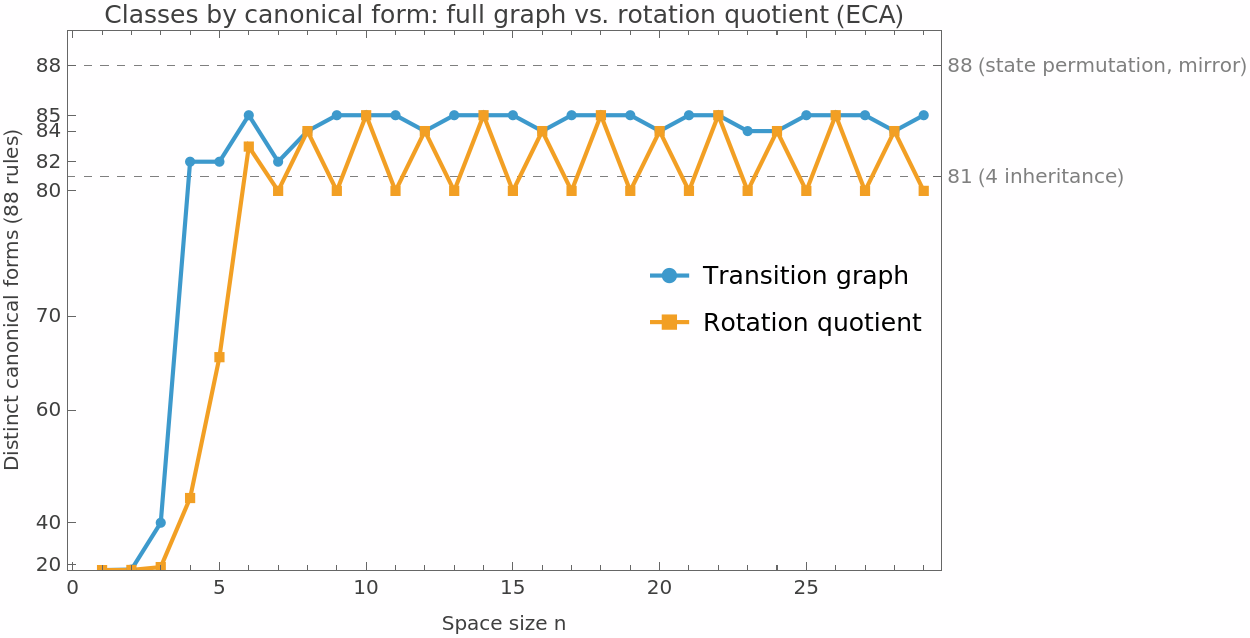
\includegraphics[width=0.85\textwidth]{canonical_classes_combined_gpu.png}
\caption{Number of canonical forms among the 88 classes with the full transition graph and the quotient by translations (the $y$ axis is on a cubic scale).}
\label{fig:canonical-rot}
\end{figure}

The partitions of the full graph and of the quotient are not nested. With odd $n$, the grouping of the full graph also occurs in the quotient, but with even $n$ each one separates pairs that the other groups. Therefore, using both canonical forms on the same space distinguishes the 88 behaviors with $n = 6, 10, 12, 14, 18, 22, 24$ and $26$. That is, a single space of 6 cells is enough if both the full graph and its quotient are used (Table~\ref{tab:canonical-rot}).

\begin{table}[H]
\centering
\setlength{\tabcolsep}{3.5pt}
\begin{tabular}{l*{12}{c}}
\hline
$n$ & 1 & 2 & 3 & 4 & 5 & 6 & 7 & 8 & 9 & 10 & 11 & 12 \\
\hline
Full & 3 & 9 & 40 & 82 & 82 & 85 & 82 & 84 & 85 & 85 & 85 & 84 \\
Quotient & 3 & 6 & 16 & 46 & 66 & 83 & 80 & 84 & 80 & 85 & 80 & 84 \\
Both    & 3 & 10 & 40 & 85 & 82 & \textbf{88} & 84 & 87 & 85 & \textbf{88} & 85 & \textbf{88} \\
\hline
\end{tabular}
\caption{Number of classes with the canonical form of the full graph, of the quotient, and of both.}
\label{tab:canonical-rot}
\end{table}

\section{Spectral methods}
\label{sec:spectral}

The methods seen so far only detect equality between rules. To obtain a gradual measure, we represent each rule as a numerical vector (embedding) derived from its transition graph, so that the distance between vectors works as a similarity index.

\subsection{Eigenvalues}

In this method we compute the eigenvalues of the adjacency matrix $A$ of the transition graph, sort them and use them as the embedding of the rule: two rules are compared through the cosine distance between their vectors. If two graphs are isomorphic, their adjacency matrices are similar through a permutation and produce the same eigenvalues, so the distance is zero. Otherwise, the distance measures how different their spectra are. This method obtains a maximum of 74 distinct behaviors (with 18 cells) in ECA.

This method has two limitations:

\begin{table}[!htbp]
    \centering
    \begin{tabular}{p{0.15\textwidth} p{0.85\textwidth}}
        Blindness to transients: &
        Each connected component has a basin made of transient trees. Since the trees only contribute zero eigenvalues, the spectrum depends only on the attractors and not on the trees. ECA rules 0 and 8 are not related by any inheritance property; however, both have a single fixed-point attractor made of all zeros, reached in 1 step with rule 0 and in at most 2 steps with rule 8, so their eigenvalues are identical. \\
        Domain dependence: &
        The number of eigenvalues equals the number of nodes $N = |\mathcal{S}|^n$, so only rules with the same number of states and the same space size can be compared.
    \end{tabular}
\end{table}

In the full graph the number of classes oscillates between 67 and 74 from $n = 8$ on, with the maximum at $n = 18$ (Figure~\ref{fig:eigen-classes}). For every size, the partition given by the canonical form is finer than the one given by the spectrum. The quotient yields fewer classes (between 56 and 63 from $n = 12$ on) because, besides the blindness to transients, it identifies each rule with its composition with the translation, such as \{15,51\} and \{170,204\}. The quotient adds no information to the spectrum: combining the 29 sizes of both graphs reaches a limit of 77.

\begin{figure}[!htbp]
\centering
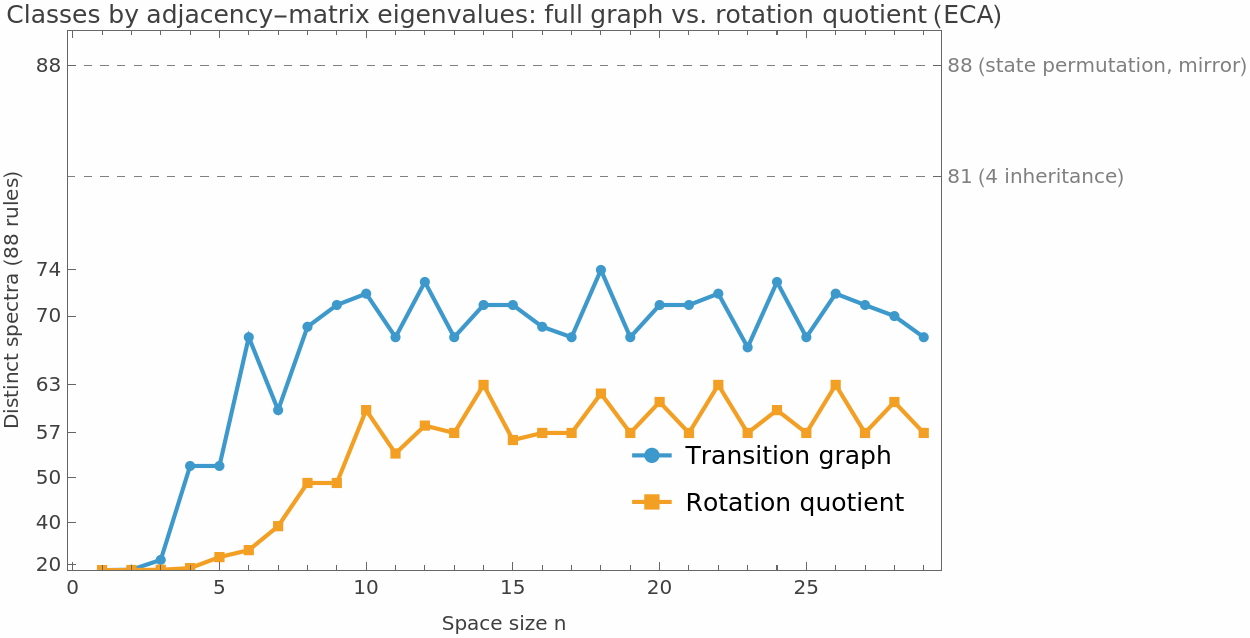
\includegraphics[width=0.85\textwidth]{eigenvalue_classes_combined_gpu.png}
\caption{Number of distinct spectra among the 88 representative rules with the full transition graph and with the quotient graph by translations.}
\label{fig:eigen-classes}
\end{figure}

The groups \{0,8\}, \{1,19\}, \{2,24,46\}, \{4,12\}, \{18,126\}, \{36,72\}, \{128,136\}, \{130,152\}, \{132,140\} and \{162,168\} have the same spectrum for every size computed. They are rules with the same cycles that differ only in their transients.

\subsection{Spectral moments}

To remove the domain dependence we propose to use spectral moments. Instead of computing the full spectrum, for each step $k = 1, \dots, K$ we measure the proportion of configurations that return to themselves after $k$ steps:
\[
  m_k = \frac{|\{x \in \mathcal{C} : F^k(x) = x\}|}{N}.
\]

The length of the vector does not depend on the number of nodes but on the window size $K$, so rules with different numbers of states, neighbors or spaces can be compared. The drawback is that $K$ must be chosen so that the relevant cycles of both graphs fall inside the window. The vectors are compared through the cosine distance, which is our similarity index.

In ECA, with the quotient graph by rotations of 14 cells and $K = 10$, we obtain 63 distinct vectors for the 256 rules. However, since $m_k$ depends only on the eigenvalues, this method inherits the blindness to transients (Figure~\ref{fig:sm-classes}).

\begin{figure}[!htbp]
    \centering
    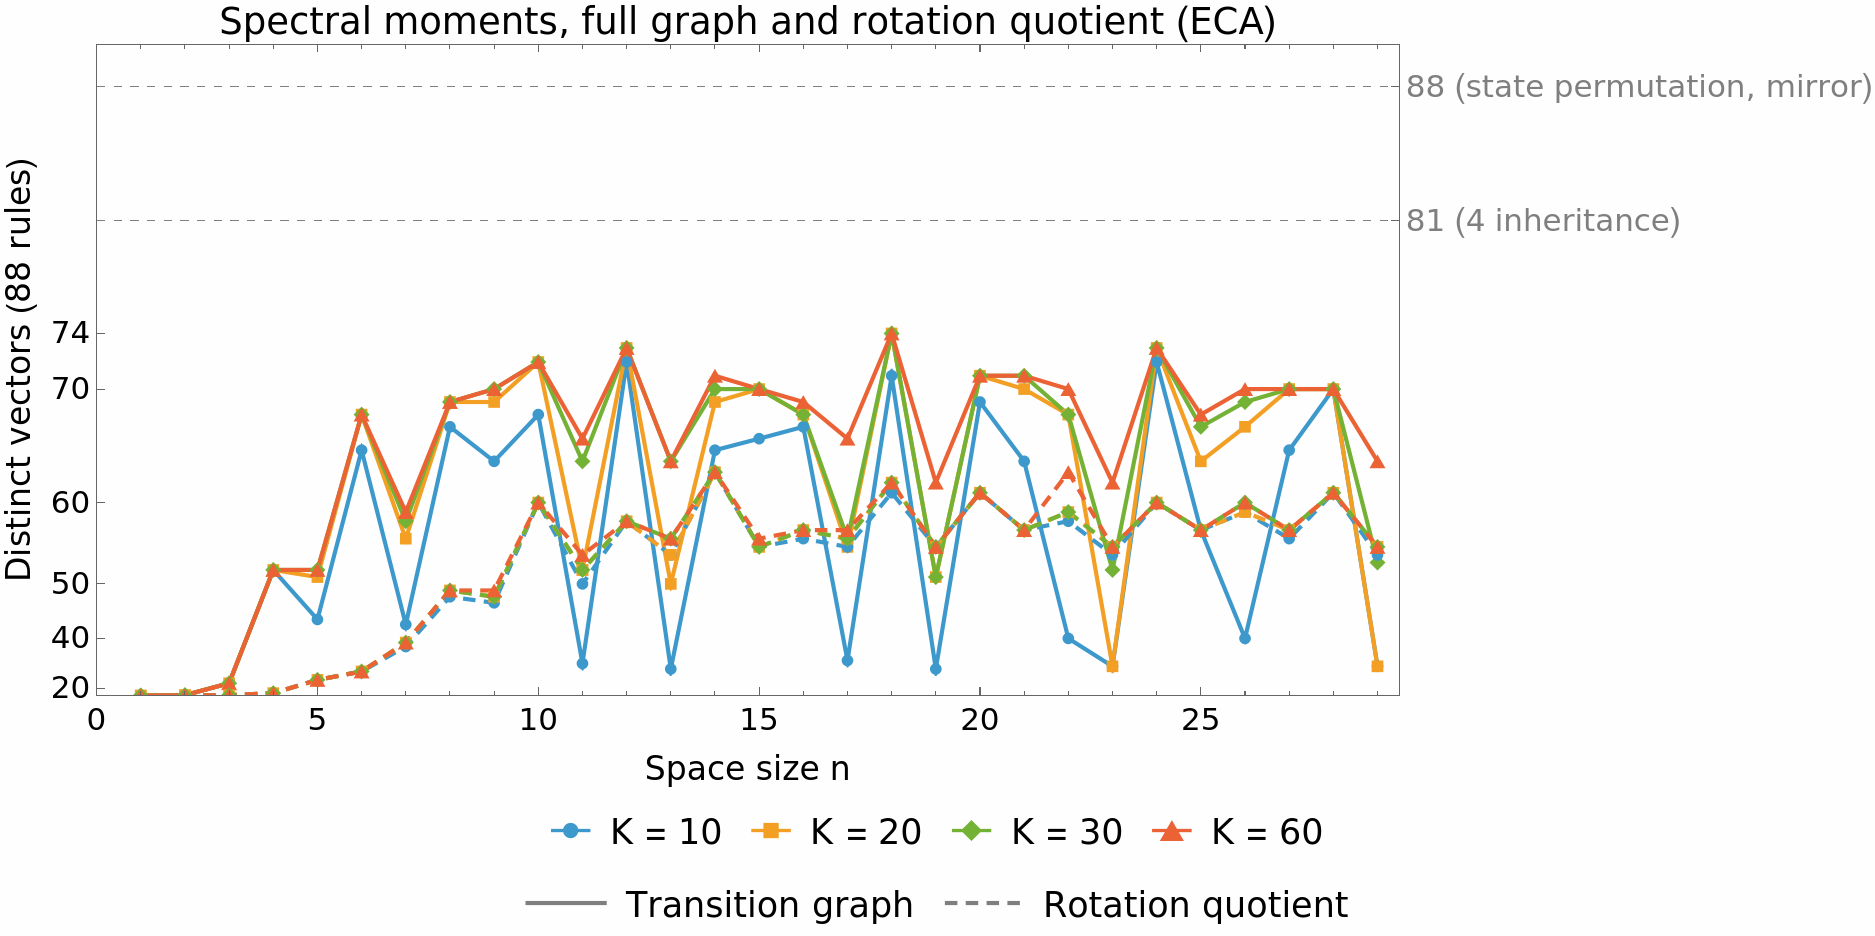
\includegraphics[width=\textwidth]{spectral_moments_classes_combined_gpu.png}
    \caption{Number of distinct spectral moment vectors among the 88 representative rules for $n = 1, \dots, 29$ and $K = 10, 20, 30, 60$, in the full graph (solid line) and in the quotient graph (dashed line).}
    \label{fig:sm-classes}
\end{figure}

A cycle of length $L > K$ is not captured by the vector. In the full graph with $K = 10$, the sizes with long cycles lose information ($n = 11, 13, 17, 19, 23$ and $29$ give between 31 and 34 classes). The sizes with many divisors give up to 72 ($n = 12$ and $24$).

In the quotient the cycles become shorter and $K$ barely matters: with $K = 10$ it finds between 54 and 63 classes from $n = 13$ on, with a maximum of 63 at $n = 14$.

Combining the 29 sizes gives 77 classes in the full graph and 68 in the quotient, the same as with the eigenvalues, for any $K$.

\subsection{Spectral moments with attractor mass}
\label{subsec:attractor_mass}

To distinguish rules such as 0 and 8, we need to measure, besides the attractors, how strongly they attract the other configurations, that is, to quantify how many configurations reach each attractor and in how many steps. The idea is that each cycle is still activated every $p$ steps, as in the spectral moments, but at each activation we also add the configurations that have already reached it.

Using the height $h(x)$ and the period $p(x)$ of each configuration, we define
\[
  \tilde{m}_k = \frac{|\{x \in \mathcal{C} : p(x) \mid k \ \text{ and } \ h(x) \le k - p(x)\}|}{N}, \quad k = 1, \dots, K.
\]
That is, a configuration counts at step $k$ if its attractor is activated at that step and the configuration had already reached it before the previous activation. Thus, cycle nodes ($h = 0$) count from the first activation ($k = p$), nodes with $1 \le h \le p$ from the second ($k = 2p$), nodes with $p < h \le 2p$ from the third, and so on.

Since every periodic configuration satisfies the condition when $p \mid k$, the vector decomposes as
\[
  \tilde{m}_k = m_k + t_k,
\]
where $m_k$ is the spectral moment and $t_k$ is the proportion of transient configurations that count at step $k$. Therefore, the new vector extends the spectral moments with the information of the basins, and keeps the advantage of having a length $K$ independent of the domain.

For example, with 5 cells ($N = 32$), rule 0 sends every configuration to zero in one step ($h \le 1$), whereas in rule 8 each block of ones leaves an isolated 1 that disappears in the next step ($h \le 2$); of the 32 configurations, 12 reach zero in at most one step. Their vectors are
\[
  \tilde{m}^{(0)} = \tfrac{1}{32}\,(1, 32, 32, 32, \dots), \qquad
  \tilde{m}^{(8)} = \tfrac{1}{32}\,(1, 12, 32, 32, \dots),
\]
which are no longer equal, even though their spectral moments are.

This method has some limitations. The resolution with which the height is measured depends on the period, since configurations are grouped in intervals of $p$ steps: with long periods, a configuration with $h = 1$ and another with $h = p$ count at the same step. Moreover, a cycle with $p > K$ is never activated.

\begin{figure}[!htbp]
    \centering
    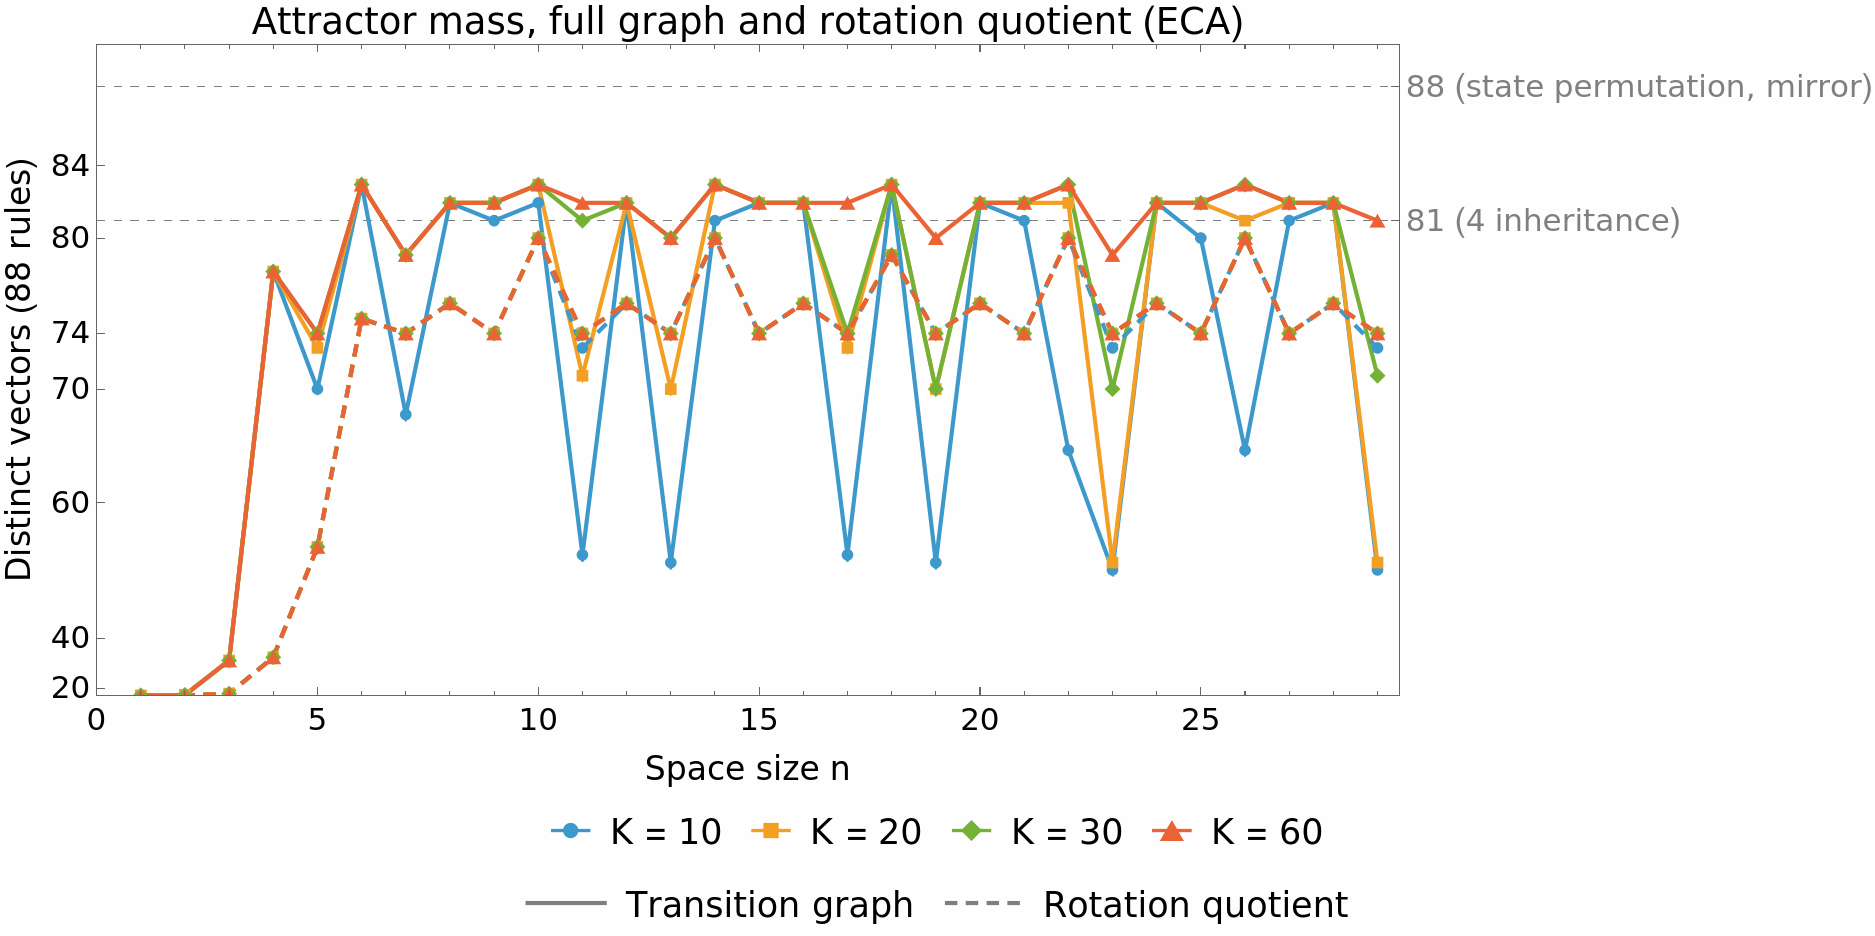
\includegraphics[width=\textwidth]{attractor_mass_classes_combined_gpu.png}
    \caption{Number of distinct spectral moment vectors with attractor mass among the 88 representative rules for $n = 1, \dots, 29$ and $K = 10, 20, 30, 60$, in the full graph (solid line) and in the quotient graph (dashed line).}
    \label{fig:am-classes}
\end{figure}

With the attractor mass the number of classes increases considerably (Figure~\ref{fig:am-classes}). In the full graph, the sizes with many divisors give between 80 and 83 classes with $K = 10$, against a maximum of 74 with the eigenvalues and 72 with the spectral moments. The sizes with long cycles still depend on the window ($n = 29$ gives 52 classes with $K = 10$ and 81 with $K = 60$). In the quotient the number of classes depends only on $n \bmod 4$ from $n = 7$ on: with $K = 60$ we obtain 74 classes if $n$ is odd, 80 if $n \equiv 2 \pmod 4$ (79 with $n = 18$) and 76 if $4 \mid n$.

Rules 0 and 8 are separated for every $n \ge 3$. Combining the 29 sizes gives 86 classes in the full graph, and two small sizes are enough (for example, $n = 3$ and $n = 6$). Only two pairs remain together. In \{1,19\} the exact heights are different (with $p = 2$, some configurations have $h = 1$ in one rule and $h = 2$ in the other), but they fall in the same interval of $p$ steps: this is the resolution limitation described above. In \{4,12\} the joint distribution of height and period is identical and the rules differ only in the shape of the trees, which only the canonical form distinguishes. The quotient, on the other hand, groups the rules that differ by a composition with the translation (\{15,51\}, \{170,204\}, \{4,12,34\}, \ldots) and only reaches 81 classes. Using the full graph and the quotient on the same size gives 87 classes with $n = 6, 10, 12, 14, 18, 22, 24$ and $26$.

Figure~\ref{fig:all-methods} and Table~\ref{tab:methods} compare all the methods. The canonical form leads in the number of classes, but the spectral moments with attractor mass are the second best method, producing up to 87 classes in total, followed by the eigenvalues and the plain spectral moments.

\begin{figure}[!htbp]
\centering
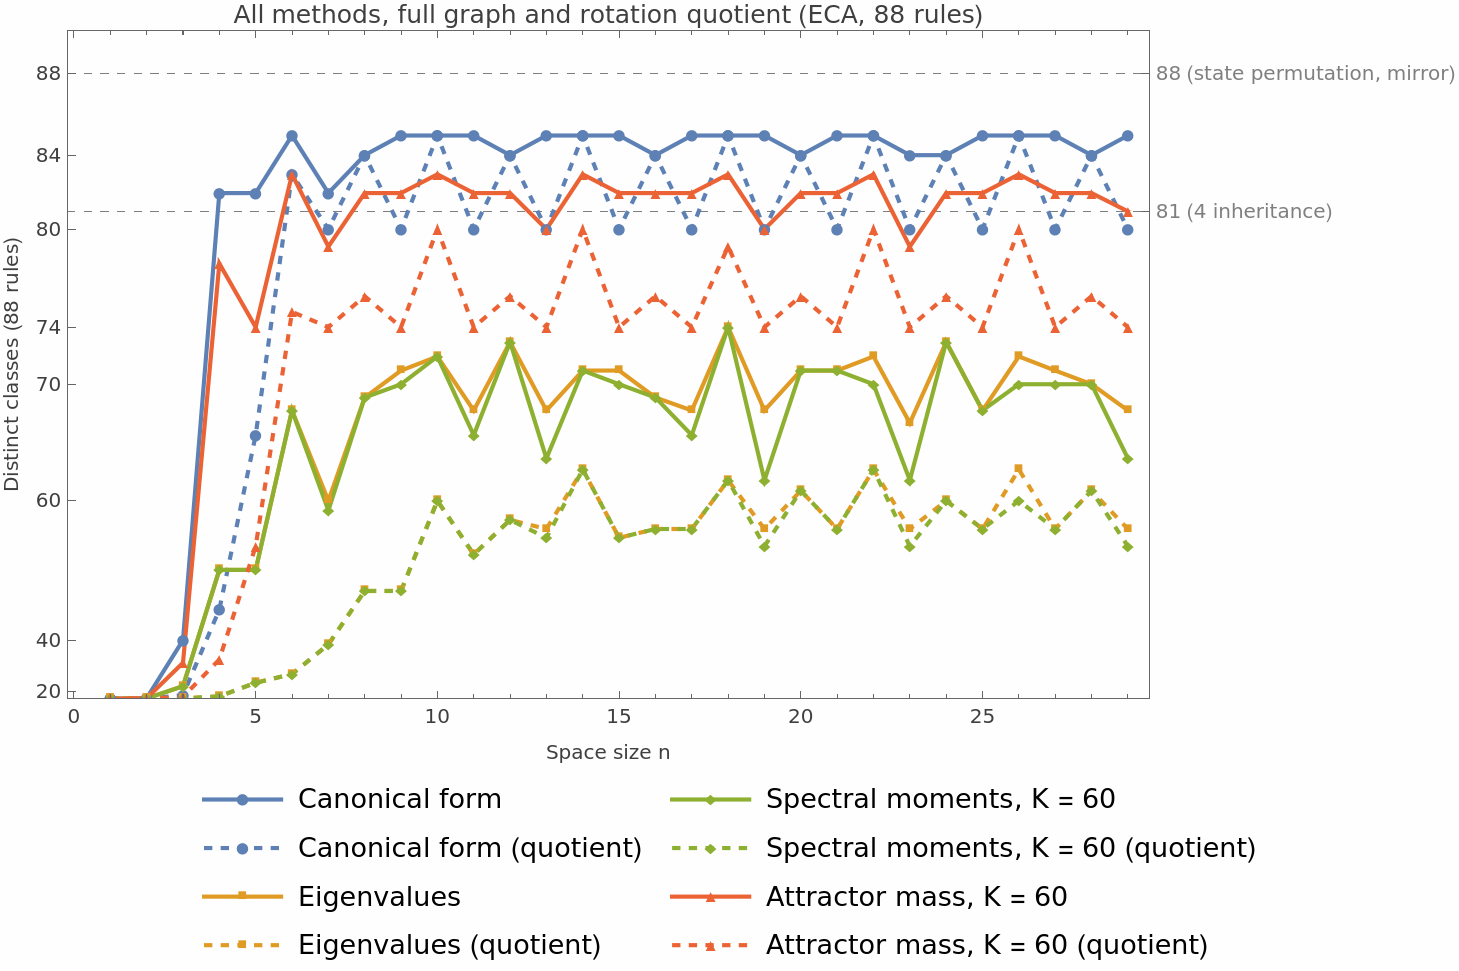
\includegraphics[width=\textwidth]{all_methods_8_classes_gpu.png}
\caption{Number of classes among the 88 representative rules with each method for $n = 1, \dots, 29$.}
\label{fig:all-methods}
\end{figure}

\begin{table}[!htbp]
\centering
\setlength{\tabcolsep}{4pt}
\begin{tabular}{lccccc}
\hline
 & \multicolumn{2}{c}{Full graph} & \multicolumn{2}{c}{Quotient} & Full \\
Method & One size & All & One size & All & + quotient \\
\hline
Canonical form & 85 & 88 & 85 & 85 & 88 \\
Eigenvalues & 74 & 77 & 63 & 68 & 77 \\
Spectral moments & 74 & 77 & 63 & 68 & 77 \\
Attractor mass & 83 & 86 & 80 & 81 & 87 \\
\hline
\end{tabular}
\caption{Maximum number of classes among the 88 representative rules. ``One size'': best $n$; ``All'': combines the 29 sizes; ``Full + quotient'': both graphs.}
\label{tab:methods}
\end{table}

\section{Experiments}
\label{sec:experiments}

In this section we evaluate the spectral moments with attractor mass with $K = 60$ and the cosine distance $d(u, v) = 1 - u \cdot v / (\|u\|\,\|v\|)$, in the full graph and in the quotient. The vectors of the rules from other domains were computed with up to $n = 12$ cells and at most 3 states ($3^{12} = 531\,441$ configurations).

\subsection{Related rules from different domains}
\label{subsec:cross-domain}

We computed the four relations of Section~\ref{sec:inheritance} between all the rules of the domains $(q, m) = (2,1)$, $(2,2)$, $(2,3)$, $(3,1)$ and $(3,2)$, together with the 3-state extension of every ECA (domain $(3,3)$), and we compare on the same space size the vectors of each pair of rules directly linked by a relation (Table~\ref{tab:cross-domain}).

\begin{table}[!htbp]
\centering
\setlength{\tabcolsep}{2.5pt}
\begin{tabular}{llrcccc}
\hline
 & & & \multicolumn{2}{c}{Pairs with $d = 0$} & \multicolumn{2}{c}{Median of $d$} \\
Relation & Domains & Pairs & Full & Quotient & Full & Quotient \\
\hline
State permutation & all except $(3,3)$ & 1010 & 1010 & 1010 & 0 & 0 \\
Mirror, odd $m$ & $(2,3)$, $(3,3)$ & 384 & 384 & 384 & 0 & 0 \\
Mirror, $m = 2$ & $(2,2)$, $(3,2)$ & 104 & 12 & 104 & 0.54 & 0 \\
Neighborhood reduction & $(2,3) \to (2,2)$ & 38 & 20 & 32 & 0 & 0 \\
 & $(2,2) \to (2,1)$ & 6 & 4 & 6 & 0 & 0 \\
 & $(3,2) \to (3,1)$ & 51 & 33 & 51 & 0 & 0 \\
State reduction & $(3,1) \to (2,1)$ & 4 & 0 & 0 & 0.008 & 0.008 \\
 & $(3,2) \to (2,2)$ & 16 & 0 & 0 & 0.015 & 0.008 \\
 & $(3,3) \to (2,3)$ & 256 & 0 & 0 & 0.083 & 0.010 \\
\hline
ECA of different classes & $(2,3)$ & 3820 & 6 & 11 & 0.33 & 0.10 \\
\hline
\end{tabular}
\caption{Distance between the attractor mass vectors of rules linked by an inheritance relation, with $n = 12$ and $K = 60$. The last row is the reference: pairs of ECA that do not belong to the same class.}
\label{tab:cross-domain}
\end{table}

With $m = 2$, the reflected neighborhood $(i-1, i)$ is $(i, i+1)$, so the mirror rule is the original one composed with a translation: the quotient graph ignores this effect, while the full graph is sensitive to the translation (median 0.54). The same happens with neighborhood reduction: if the remaining neighbors keep their position, the reduced rule has the same global function and the distance is 0, and if the neighborhood is shifted, the global function changes by a translation. The only ECA reductions with positive distance in the quotient are those of rules that depend on non-contiguous neighbors ($\sigma_{i-1}$ and $\sigma_{i+1}$), because with even $n$ the ring splits into two sublattices of $n/2$ cells; with odd $n$ (for example, $n = 11$) the distance is 0.

State reduction never gives distance 0. The extension of a rule to $q + 1$ states preserves its cycles, but adds $(q+1)^n - q^n$ Gardens of Eden, which with $n = 12$ make up 99.2\% of the configurations. Even so, the extension largely preserves the order of the distances (Spearman correlation of 0.47 in the full graph and 0.76 in the quotient), although the original rule is the ECA closest to its extension in only 5 of the 88 cases (10 in the quotient). In contrast, the plain spectral moments do give distance 0, because the extension has the same cycles and only the normalization changes.

Finally, the distance between rules 0 and 8 is positive for every $n \ge 3$ and grows with $n$ (0.0072 with $n = 12$) until it stabilizes at 0.0085 with $n = 29$. The rules closest to 0 are not 8 but 4, 12 and 200 ($d \le 0.0004$), which reach a fixed point in a single step.

\subsection{One rule on spaces of different sizes}
\label{subsec:sizes}

We compare each of the 88 ECA with itself over all pairs of sizes $n \neq n'$ with $n, n' \in \{8, \dots, 29\}$. The median distance between the vectors of the same rule is 0.098 in the full graph and 0.001 in the quotient, against 0.47 and 0.23 between different rules of the same size. However, since many rules have very close neighbors, a rule is identified (its nearest vector at the other size is its own) in only 25\% of the cases in the full graph and 33\% in the quotient (Figure~\ref{fig:size-id}).

\begin{figure}[!htbp]
\centering
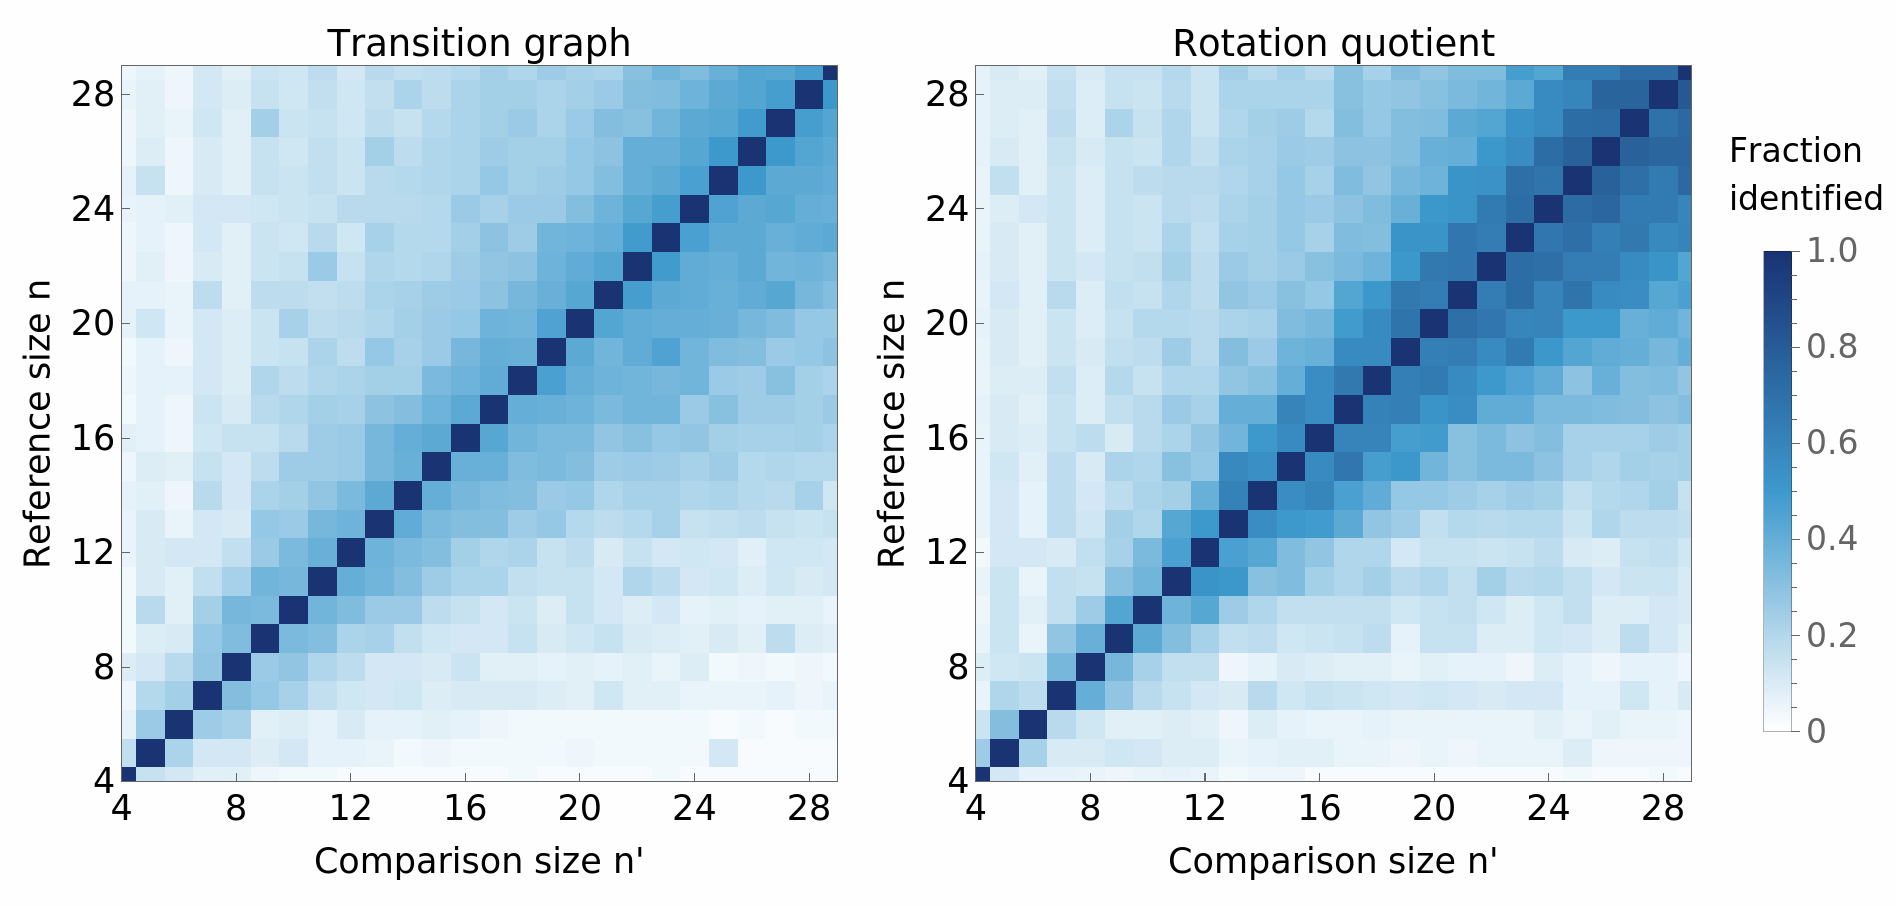
\includegraphics[width=0.85\textwidth]{attractor_mass_size_identification.png}
\caption{Fraction of the 88 ECA that are identified between sizes $n$ and $n'$ ($K = 60$).}
\label{fig:size-id}
\end{figure}

Stability depends on the dynamics of each rule. Negation (51) and identity (204) are identified for every pair of sizes and, in the full graph, so are other rules whose vector barely changes with $n$, such as 0, 8, 54, 62 and 94, in more than 80\% of the pairs. Shift rules (for example 2, 24, 34, 42, 56 and 170) are never identified in the full graph, because the length of their cycles depends on the divisors of $n$; the quotient improves them (identification ranges from 25\% of the pairs for rule 2 to all of them for rule 170), but the chaotic and additive rules (18, 60, 122, 126, 146 and 150) are almost never identified. Therefore, the comparison between different sizes is only reliable for rules whose attractors do not depend on $n$, and in general it is better to compare on the same size.

\subsection{Clustering of the ECA}
\label{subsec:clustering}

Finally, we cluster the 88 representative ECA with $n = 12$ and $K = 60$. We tried $k$-medoids and hierarchical clustering with 4 and 5 clusters; the best partition is the $k$-medoids one with 4 clusters (silhouette 0.70). Figure~\ref{fig:clusters} shows a projection of the clusters onto two dimensions by classical multidimensional scaling, which preserves 77\% of the variance. The clusters are separated by the dominant period of their attractors (Table~\ref{tab:clusters}): the first gathers rules that send almost everything to fixed points, with a vector that saturates close to 1, such as the null rules and the rules with many fixed points; the second, rules whose attractors shift, with cycles of period $n$ or $2n$ that are only activated at $k = 12, 24, \dots$; the third, rules with period-2 attractors, whose vector alternates between even and odd steps, such as negation and the additive rules; and the fourth, rules with long cycles.

\begin{figure}[!ht]
\centering
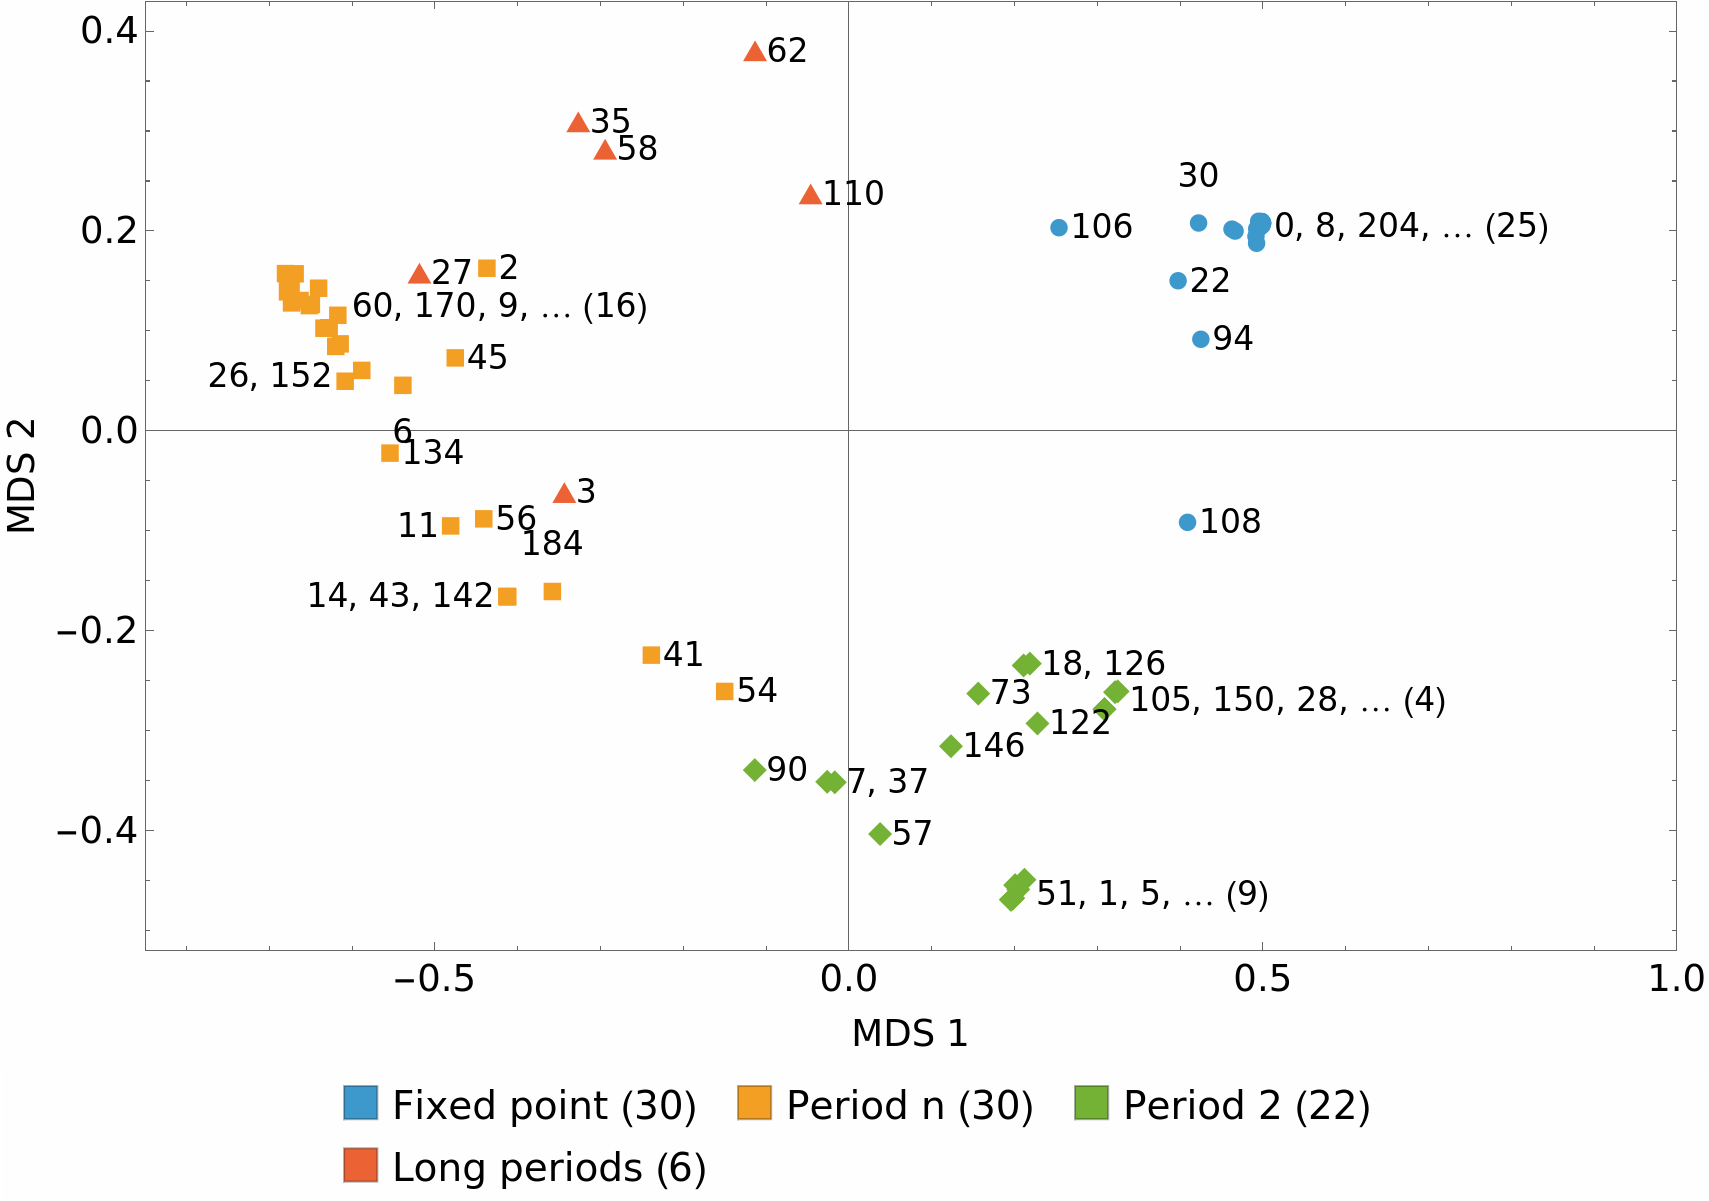
\includegraphics[width=0.8\textwidth]{attractor_mass_clusters_n12.png}
\caption{Two-dimensional projection of the clustering of the 88 representative ECA by attractor mass ($n = 12$, $K = 60$, $k$-medoids with 4 clusters). Very close points share a label, with the number of rules in parentheses.}
\label{fig:clusters}
\end{figure}

\begin{table}[!ht]
\centering
\setlength{\tabcolsep}{4pt}
\begin{tabular}{p{0.2\textwidth} p{0.1\textwidth} p{0.63\textwidth}}
\hline
Cluster & Period & Rules \\
\hline
Fixed point (30) & 1 (29) & 0, 4, 8, 12, 13, 22, 30, 32, 36, 40, 44, 72, 76, 77, 78, 94, 104, 106, 108, 128, 132, 136, 140, 160, 164, 168, 172, 200, 204, 232 \\
Period $n$ (30) & 12 (27) & 2, 6, 9, 10, 11, 14, 15, 24, 25, 26, 34, 38, 41, 42, 43, 45, 46, 54, 56, 60, 74, 130, 134, 138, 142, 152, 154, 162, 170, 184 \\
Period 2 (22) & 2 (16) & 1, 5, 7, 18, 19, 23, 28, 29, 33, 37, 50, 51, 57, 73, 90, 105, 122, 126, 146, 150, 156, 178 \\
Long periods (6) & 24 (3) & 3, 27, 35, 58, 62, 110 \\
\hline
\end{tabular}
\caption{Clusters of Figure~\ref{fig:clusters}. Period: the dominant period, which gathers the most configurations within the window, and in parentheses the number of rules of the cluster in which it dominates.}
\label{tab:clusters}
\end{table}

However, the chaotic rules do not form a cluster of their own, for two reasons. In some of them, most configurations reach cycles with period greater than $K$, which are never activated, and almost all the others reach a fixed point; since the cosine distance discards the magnitude of the vector, they end up in the fixed-point cluster (e.g., rule 30). In others, most do reach a fixed point (e.g., rules 22 and 106).

\section{Conclusions}
\label{sec:conclusions}

The four inheritance relations connect rules from different domains and reduce the 256 ECA to 81 classes. The canonical form of the transition graph exactly distinguishes the 88 classes under permutation and mirror with a single space of 6 cells if both the full graph and its quotient by translations are used, but it gives a binary comparison limited to rules of the same domain.

The eigenvalues and the spectral moments only see the attractors: they do not separate rules that differ in their transients, such as 0 and 8, and they stop at 77 classes. The spectral moments with attractor mass keep their fixed length and add the information of the basins: they distinguish 86 of the 88 classes (87 together with the quotient) and separate rules 0 and 8, although with a small distance (0.007 with $n = 12$) because the difference lies in the first steps of a vector that saturates.

Across domains, the attractor mass gives zero distance to the relations that preserve the transition graph and, in the quotient, also to those that change it by a translation; thus, making the neighbors contiguous seems to preserve the behavior (modulo translations, except for non-contiguous neighborhoods on spaces of even size), but the exact comparison is to keep the neighbors at their original positions: in that case the global function is the same and the distance is always zero, as when an end neighbor is removed. State reduction is not identified, because the configurations with the new state dominate the normalization; the plain spectral moments, in contrast, are invariant under it. Moreover, the vector depends on the size of the space, so it is better to compare on the same size. With that precaution, the distance groups the ECA into four families according to the dominant period of their attractors, although the chaotic rules are scattered because their long cycles do not fit in the window.

Future work includes: normalizing the attractor mass so that it is invariant under state reduction, for example by restricting it to the configurations that survive the first step; giving more weight to the first steps and keeping the magnitude of the vector; choosing the space size and the window $K$ systematically; checking whether the similarity holds when the neighbors are made contiguous; studying dimension reduction; and extending the comparison to larger domains through sampling.

%
% ---- Acknowledgments and disclosure ----
\begin{credits}
% Acknowledgments are omitted for the double-blind review; see credits.tex.
\subsubsection{\discintname}
The authors have no competing interests to declare that are relevant to
the content of this article.
\end{credits}

%
% ---- Bibliography ----
% Copy of splncs04 that numbers the references in order of citation.
\bibliographystyle{splncs04-unsorted}
\bibliography{references}
%
\end{document}
